% \begin{equation*}
%     \beta(s=0) \overset{\mathrm{def}}{=}  \beta_0 = e^{- \kappa F(0)},
%     \hspace{0.5cm} \Rightarrow \hspace{0.5cm}
%     \kappa = \frac{\ln 1/\beta_0}{F(0)},
% \end{equation*}
% где $1-\beta_0$ -- глубина доплеровского провала.

Контрастность\footnote{
    Отношение высоты лэмбоского пика к глубине доплер. провала.
}  спектроскопии $K$:
\begin{equation*}
    \frac{\sub{I}{out}}{\sub{I}{int}} = \exp\left[
        - \kappa F(s, \nu)
    \right], 
    \hspace{0.5cm} \Rightarrow \hspace{0.5cm}
    K(s)  = 
    \frac{\beta_0^{F(s)/F(0)}-\beta_0}{1-\beta_0},
\end{equation*}
где $\beta \overset{\mathrm{def}}{=}  \sub{I}{out}/\sub{I}{in}$, подразумеваем $\nu = \nu_\text{рез}$, $\beta_0 \overset{\mathrm{def}}{=} \beta(s=0)$.

\begin{figure}[h]
    \centering
    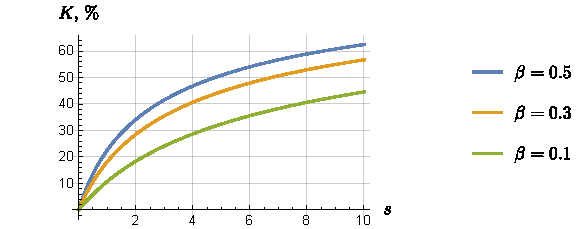
\includegraphics[width=0.81\textwidth]{"D:\\Kami\\git_folder\\notes_5sem\\rqc\\saturation_spectr_simulation\\K.pdf"}
    \caption{Оценка контрастности при различных значениях $\beta$, как функция от $s$}
    %\label{fig:}
\end{figure}